\section{Assigment 3}

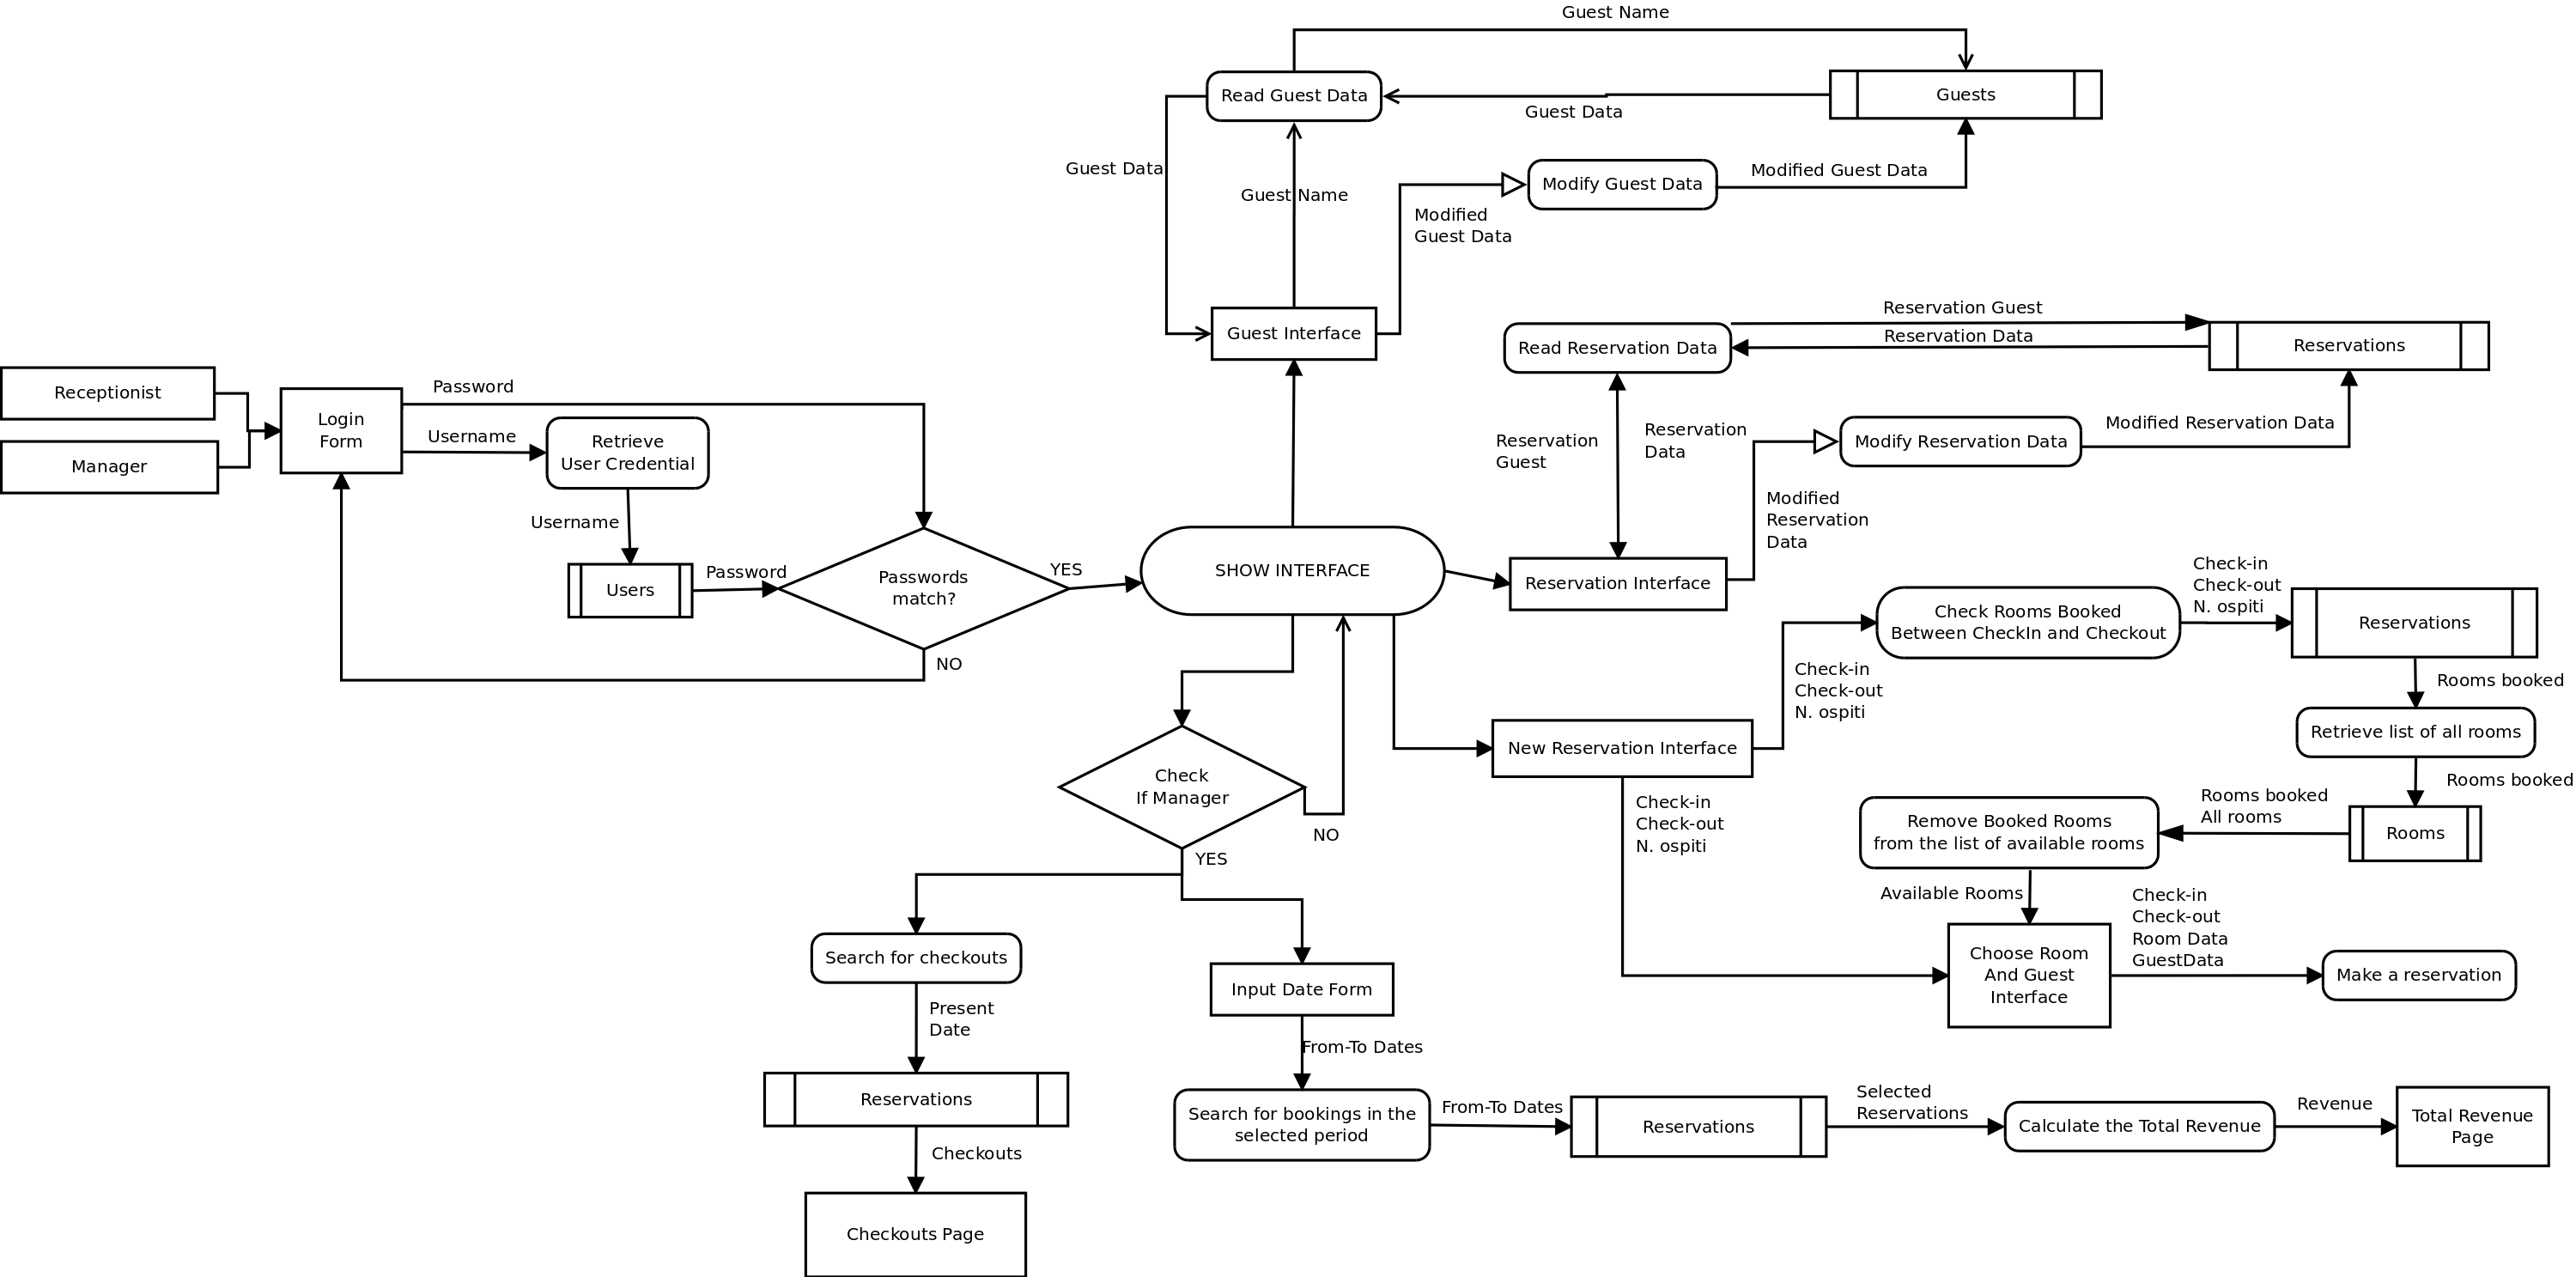
\includepdf[angle=90]{Diagram3}

\subsection{Elementary Process}

\begin{description}
  
  \item[Receptionist :] \hfill \\ user that cannot see the manager's reserved part of the system

  \item[Manager :] \hfill \\ user that has a full access to the system
    
  \item[Login Form :] \hfill \\ a form to login the system
    
  \item[Retrive User Credential :] \hfill \\ retrive the user credential for the users database table
    
  \item[Users (database) :] \hfill \\ where the user credential and information are stored

  \item[Password Match? :] \hfill \\ check if the user credential input is in the users database table

  \item[Show Interface :] \hfill \\ open the homepage of the system
    
  \item[Guest Interface :] \hfill \\ a page where the guest information are managed

  \item[Read Guest Data :] \hfill \\ a function to read all the information about the guest
    
  \item[Guest (database) :] \hfill \\ where all guest informations are stored
    
  \item[Modify Guest Data :] \hfill \\ a function to modify all or a part of the information about a guest
    
  \item[Reservation Interface :] \hfill \\ a page where the reservation information are managed
    
  \item[Modify Reservation Data :] \hfill \\ a function to modify the reservation data
    
  \item[Reservations (database) :] \hfill \\ where all the reservation are stored
    
  \item[Read Reservation Data :] \hfill \\ a function to read the reservation data
    
  \item[New Reservation Interface :] \hfill \\ a page where the user can do a new reservation

  \item[Check Rooms Booked Between Checkin and Checkout :] \hfill \\ a function to see the booked room in a period
    
  \item[Retrive List Of All Rooms :] \hfill \\ a function to get the list of all the hotel'92s rooms
    
  \item[Rooms (database) :] \hfill \\ where the rooms'92 informations are stored
    
  \item[Remove Booked Rooms From The List of Available Rooms :] \hfill \\ a function to remove the booked rooms from the list of the available rooms

  \item[Choose Room And Guest interface :] \hfill \\ a page where the user can choose the room and input the guest information
    
  \item[Make A Reservation :] \hfill \\ a function to make a reservation

  \item[Check If Manager :] \hfill \\ a function to see if a user is a manager

  \item[Search for Check-OUTs :] \hfill \\ a functions to see all the check-out of that specified day

  \item[Check-OUTs Page :] \hfill \\ a page where to see all the check-out
    
  \item[Input Date Room :] \hfill \\ a function to input the room information

  \item[Search For Bookings In The Selected Period :] \hfill \\ a function to search for booking 

  \item[Calculate The Total Revenue :] \hfill \\ a function to calculate the total ravenue

  \item[Total Revenue Page :] \hfill \\ a page to see the total revenue

\end{description}

\subsection{Data Structures}
  
\begin{description}
    
  \item[username:] \hfill \\ The indentifier used by the manager or receptionists to login 
    
  \item[password:] \hfill \\ The secret word used to verify the user's identity
    
  \item[Guest Name:] \hfill \\ Name of a guest searched in the database
    
  \item[Guest Data:] \hfill \\ All the information of a guest founded in the database
    
  \item[Modified Guest Data:] \hfill \\ Information modified by the user updating the guests data in the database

  \item[Reservation Guest:] \hfill \\ The ID of the guest NEED UPDATE! 
    
  \item[Reservation Data:] \hfill \\ All the information of a reservation founded in the database
    
  \item[Modified Reservation data:] \hfill \\ Information modified by the user updating the reservation data in the database

  \item[Check In/ Check Out:] \hfill \\ The data of arriving and departuring of a guest used to check the avaliability of the rooms in that period
    
  \item[Rooms booked:] \hfill \\ all the rooms not available for the indicated period
    
  \item[Available rooms:] \hfill \\ All the rooms available for the indicated period
    
  \item[All room:] \hfill \\ The list of all the room in the Hotel
    
  \item[Room Data:] \hfill \\ All the information of a room founded in the database
    
  \item[Checkouts:] \hfill \\ The reservation founded that end today
    
  \item[From/to dates:] \hfill \\ a period selected by the manager to show the reveneues in that period
    
\end {description}
